
\documentclass[12pt,english]{article}
\usepackage[T1]{fontenc}
\usepackage[latin9]{inputenc}
\usepackage{geometry}
\geometry{verbose,tmargin=1.5cm,bmargin=1.5cm,lmargin=1.5cm,rmargin=1.5cm}
\usepackage{babel}
\usepackage{graphicx}
\usepackage{amsmath}
\usepackage{amssymb}
\date{}
\begin{document}

\title{Information Sources with Combined Outputs}

\maketitle

\section*{1 Mathematical Formulation}

We consider an optimization problem that combines multiple independent
information sources,
\[
\mbox{max}_{x\in A}g\left(x\right):=\mbox{max}_{x\in A}g\left(f_{1}\left(x\right),\ldots,f_{k}\left(x\right)\right)
\]

where $A$ is the feasible compact set and $f_{1},\ldots,f_{k}$ are continuous
functions (see Figure~\ref{fig:fig1}). 

\begin{figure}[htp]
\centering
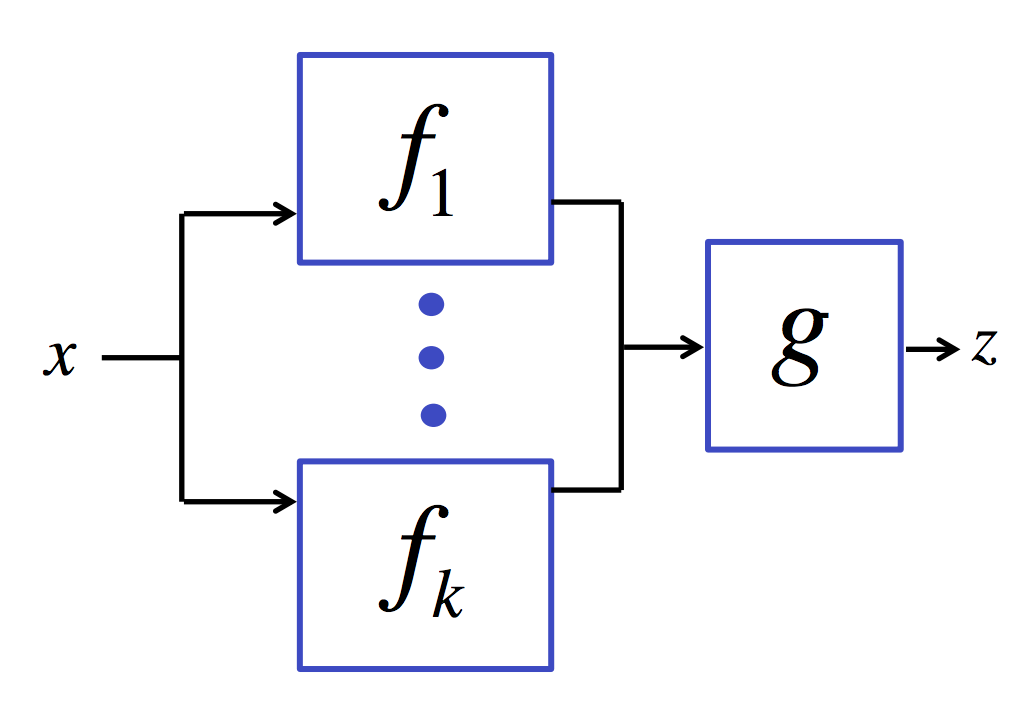
\includegraphics[width=.5\textwidth]{01.png}
\caption{Diagram of the problem}
\label{fig:fig1}
\end{figure}

\section*{2 Applications}



\subsection*{I Machine Learning.}

We have many terabytes of training data $\left\{ \left(x_{i},y_{i}\right)\right\} _{i=1}^{N}$
where $\left\{ x_{i}\right\} _{i=1}^{N}$ are the inputs and $\left\{ y_{i}\right\} _{i=1}^{N}$
are the outputs. 


\paragraph*{Training Machine Learning Models}

We have a machine learning model (e.g. logistic regression) that depends
on a vector of parameters $\alpha$. Our data is spread across $k$
disks. 

We want to choose $\alpha$ that maximizes the log-likelihood 
\begin{eqnarray*}
g\left(\alpha\right) & = & \sum_{s=1}^{k}\sum_{i\in\mbox{disk}_{s}}\mbox{log }p\left(y_{i}\mid x_{i},\alpha\right)\\
 & = & \sum_{s=1}^{k}f_{s}\left(\alpha\right)
\end{eqnarray*}
where 
\[
f_{s}\left(\alpha\right)=\sum_{i\in\mbox{disk}_{s}}\mbox{log }p\left(y_{i}\mid x_{i},\alpha\right)
\]



\paragraph*{Cross-Validation}

We have a set of models $f\left(x,\alpha\right)$ indexed by the parameter
$\alpha$ (e.g. maximum depth of decision trees). In K-Fold cross validation, we split the data into K equally
sized sets. We denote by $\hat{f}^{-k}\left(x\right)$ the fitted
function, estimated with the $k$th set removed. We want to choose
$\alpha$ that minimizes
\begin{eqnarray*}
\mbox{CV}\left(\hat{f},\alpha\right) & = & \frac{1}{N}\sum_{i=1}^{N}L\left(y_{i},\hat{f}^{-k\left(i\right)}\left(x_{i},\alpha\right)\right)
\end{eqnarray*}
where $L$ is the loss function and $k\left(i\right)$ is the set
where $x_{i}$ is for $i\in\left\{ 1,\ldots,N\right\} $. Here each
$L\left(y_{i},\hat{f}^{-k\left(i\right)}\left(x_{i},\alpha\right)\right)$
is an information source.


\subsection*{II Simulation Optimization}

We want to solve 
\[
\mbox{max}_{x}\mathbb{E}\left[f\left(x,\omega\right)\right]
\]
where $f$ is a stochastic simulator, $\omega$ is the randomness
with a known probability distribution $p$.

We define the information sources as $f_{s}\left(x\right):=f\left(x,\omega_{s}\right)$
and 
\begin{eqnarray*}
g\left(x\right) & = & g\left(f_{1}\left(x\right),\ldots,f_{k}\left(x\right),\ldots\right)\\
 & = & \sum_{s}p\left(w_{s}\right)f_{s}\left(x\right)
\end{eqnarray*}
if $\omega$ takes countable values, $\omega_{1},\ldots,\omega_{k},\ldots$. 

If $\omega\in C$ takes uncountable infinite values, then 

\[
g\left(x\right)=\int_{w}p\left(\omega\right)f_{s}\left(x,\omega\right)d\omega.
\].

\section*{3 Value of Information Functions}

We place Gaussian processes on $f_{1},\ldots,f_{k}$. Depending on the problem and the kernels of the Gaussian processes, we may have a Gaussian process on $g$.

We define the value of information functions as

\[
V_{n}\left(x,h\right)=\mathbb{E}\left[\mbox{max}_{z}a_{n+1}\left(z\right)-\mbox{max}_{z}a_{n}\left(z\right)\mid x_{n+1}=x,h\left(x\right)\right]
\]

where $h\in\left\{ f_{1},\ldots,f_{k}\right\} $.


\section*{4 Algorithm}

\begin{enumerate}
\item (First stage of samples) Use maximum likelihood or maximum a posteriori estimation to fit the
parameters $\left(\mu_{0}^{1},\Sigma_{0}^{1}\right),\left(\mu_{0}^{2},\Sigma_{0}^{2}\right),\ldots,\left(\mu_{0}^{k},\Sigma_{0}^{k}\right))$ of the GP prior on $f_{1},\ldots,f_{k}$, respectively. We denote the parameters of the GP on $g$ by $a_{0},b_{0}$.\\
 \textrm{}\\
\item (Main stage of samples) For $n\leftarrow0$ to $N$ do
\begin{enumerate}
    \item Update our joint Gaussian process posterior on $g$ using all samples by time $n$.\\
    \textrm{}\\
\item Solve $\left(x_{n+1},h_{n+1}\right)\in\mbox{arg max}_{x\in A,h\in\left\{ f_{1},\ldots,f_{k}\right\} }V_{n}\left(x,h\right)$.\\
\textrm{}\\
\item Evaluate $h_{n+1}\left(x_{n+1}\right)$\\
\textrm{}\\
\end{enumerate}
\item Return $x^{*}=\mbox{arg max}_{x}a_{N+1}\left(x\right)$.
\end{enumerate}



\end{document}
